\section{Remove}
\subsubsection{Community detection thresholds}

\subsection{Observations from Fortunato}

\subsection{Performance on PSP network}
\label{sec:Performance on PSP network}
See table~\ref{tab:modularity and group sizes xtable} 

code \url{source('~/RProjects/group_sizes/R/make_clusterings/make_clusterings.R')}


Check that the volume is equal to 2 x the edge count  TRUE 

erable variation in group size. Some methods give rise to very extreme group size values with a large number of size 1 groups or a small number of very large groups. There is some reason to believe (LFR) that in empirical networks there is a power law distribution of group size however there are some features we would like in the community detection algorithm. For the reasons in section (GSA) we would like communities of a reasonable (15 or more for example) size to avoid the signal being dominated by a small number of genes or the sample being too small to represent a group. We would however like that the number of genes we exclude on size criteria (either too large or too small) should not be a disproportionately large part of the PSP. In this way we also want to avoid very large groups. There is evidence that groups of around 100 have been shown to have the best (lowest Leskovec) conductance and these are suitable sizes for GSA (also see section~\ref{sec:optimal community size}. Very large groups also have the potential for confounding where more than one function dominates the effect\cite{de2016statistical} although it may be desirable for reasons I mention in the discussion to on occasion use large groups to partition the PSP into smaller parts for subsequent analysis of to find if signal belongs to a specific part of the graph (such as the core). 

 




We want to therefore chose a clustering method that performs well on benchmarks, gives reasonable looking group sizes on the PSP and does not result in a large number of genes being excluded. This is not unreasonable as I will return to in the discussion given that the concept of ground truth in networks is not absolute and what we want is a division that is useful. The method should also have a reasonable conductance for the groups that are of the appropriate size which we will see if we examine the community statistics following Fortunato (cross ref section~\ref{sec:Fortunato community statistics}). 


\subsubsection{Results infomap group}
\label{sec:infomap_results}

Infomap discovers 171 communities. Group size  Min. 2.00, 1st  Qu.5.00,   Median 8.00,     Mean 20.2,2 3rd Qu. 13.00 ,  Max. 1228.00

The partition results in a large number of small communities. 

The modularity of the partition is 0.275.
 \todo{mean conductance of louvain,spectral and infomap}
\subsubsection{ InfoMap Result PSP}
On the PSP there are 171 groups the majority less than fifteen members in size, the median group size is 9 and mean 20.2. THe largest group is 1228 and the next largest 130. The conductance of the largest group is low compared to mean group conductance at 0.255 OTHER WAY ROUND  suggesting this large group is not very cohesive and the clustering may be suboptimal for our purposes. 




\begin{figure}
    \centering
    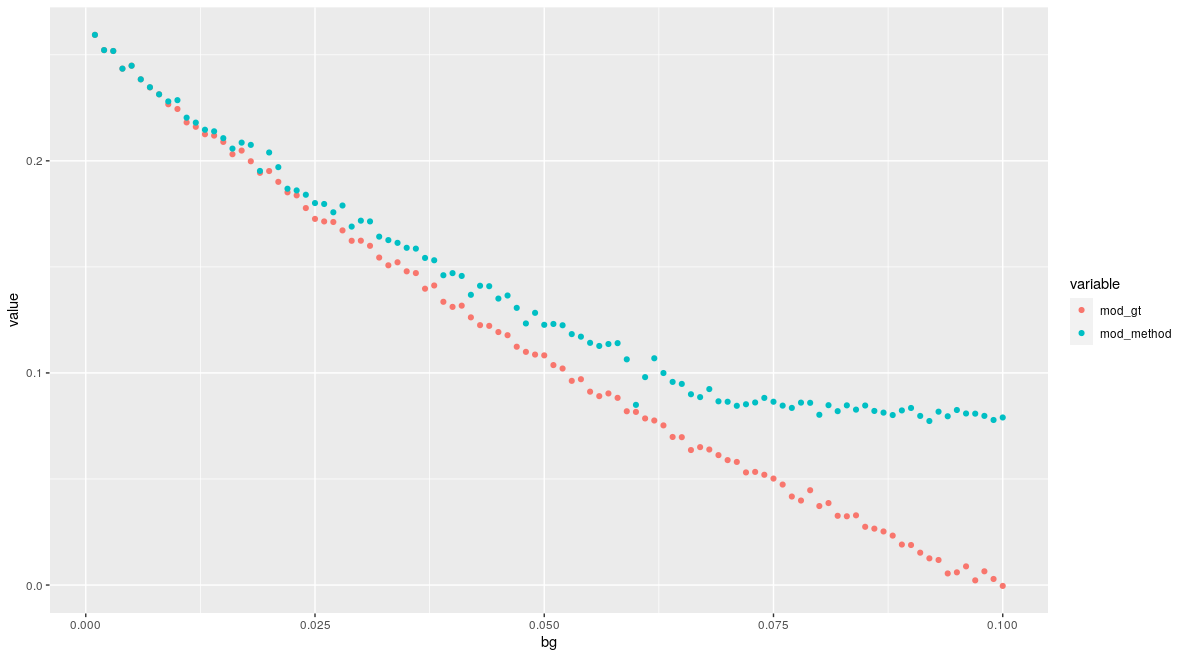
\includegraphics[width=\textwidth]{images/Rplot_rough_modularity_lou_ground_truth.png}
    \caption{Modularity group SBM louvain as approaches resolution limit. plot is p on x axis}
    \label{fig:my_rough_louvain modularity}
\end{figure}

\begin{figure}
    \centering
    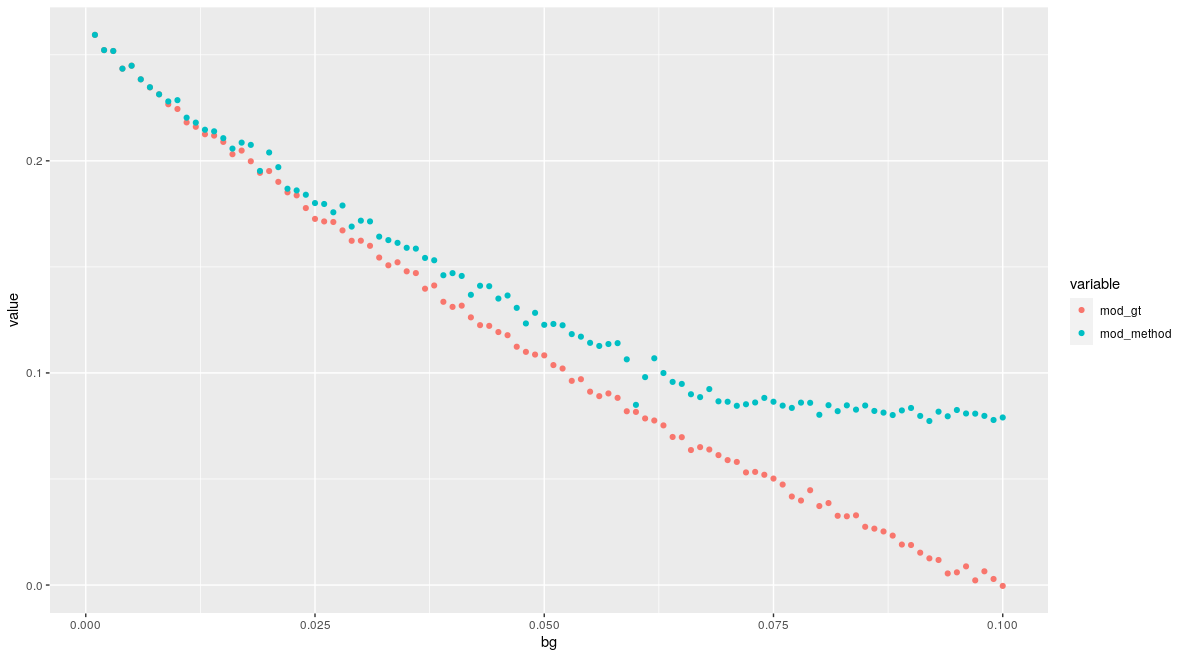
\includegraphics[width=\textwidth]{images/Rplot_rough_modularity_lou_ground_truth.png}
    \caption{Modularity group SBM louvain as approaches resolution limit. plot is p on x axis}
    \label{fig:my_rough_louvain modularity}
\end{figure}


\begin{figure}
    \centering
    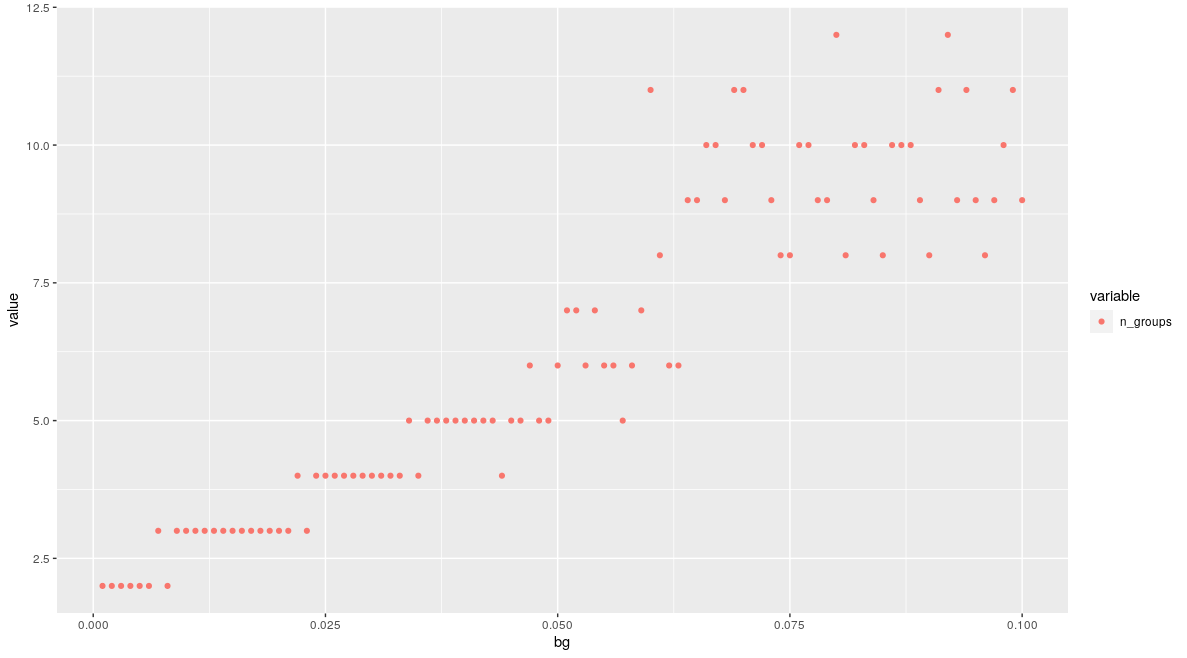
\includegraphics[width=\textwidth]{images/Rplot_group_size_rough_louvain_sbm.png}
    \caption{2 group SBM group size louvain as approaches resolution limit. plot is p on x axis see \url{source('~/RProjects/group_sizes/R/sbm_benchmark/graph/graph_performance_multi.R')}}
    \label{fig:my_rough_louvain group size}
\end{figure}


\subsection{tmp:out}
\section{Methods for paper}
\label{sec: community detection methods from paper}
To study the effect of synaptic network structure on the genetics of cognitive ability and educational attainment we have used a discovery and replication cohort design. To understand how the structure of the PSP might affect the genetic architecture of these complex phenotypes, we first tested if there was an association between measures of the influence of individual vertices (gene) in the graph (degree), and their significance in GWA studies. 
Next, we used GSA to test whether the genes encoding proteins forming community structures in the network were significantly associated with differences in intelligence or educational attainment. 

\paragraph{tmp:rephrase?}
The spectral clustering algorithm and Louvain algorithm produce communities of less disparate size although the Louvain clusters are large. \todo{graph of conductance versus community sizes}


\paragraph{tmp:paste}
($\gamma$=degree exponent,$\beta$=community exponent)
($\tau_1$ and $\tau_2$ respectively in the NetworkX implementation\cite{hagberg2008exploring})

A degree and community structure are generated using the parameters provided and each node is then randomly assigned to a community and accepted if their internal degree (number within community links which is governed by $\mu$) is less than the size of the community. Nodes which do not fit into communities are not assigned. In subsequent iterations unassigned nodes can dislodge a random node from the community and the network is rewired keeping the degree of each node constant but changing the balance of within and outwith community links to satisfy the $\mu$ constraint. 


As figure~\ref{fig:boxplot group size lfr clustering methods} shows the spectral algorithm matches the ground truth community sizes reasonably well considering that the LFR using average degree has a minimum community size of 16 and spectral clustering has 34 communities of size less than fifteen however excluding these results in a loss of only 2.02\% of the genes (compared with 47.56 for MCL table~\ref{tab:Group sizes compared with ground truth LFR 3457 PSP like benchmark1}). A community equal to one could be considered in a way analogous to not assigning a community number to it. 24 entries equal to 1. \footnote{Code at \url{source('~/RProjects/python_benchmarks/R/make_table_lfr_benchmark_group_sizes.R')}}
\footnote{Python code to generate the LFR model and test it is at \url{/home/grant/Projects_/Python/venvs/Create_LFR_similar_to_PSP.ipynb} this is on red bionic beaver machine}

